\subsection{Søgemodul}
\label{sub:s_searchmodul}

Søgemodulet har til opgave at søge i databasen og præsentere resultaterne.


\subsubsection{Funktionalitet}

Søgemodulet giver mulighed for at søge efter brugere i programmets database. Flere søgekriterier kan benyttes på samme tid for at filtrere i resultaterne. Flere informationer om en bruger kan ses ved at dobbeltklikke på brugeren i resultatlisten.

\subsubsection{Implementation}

Følgende afsnit beskriver \cref{fig:soegemodul}. Når et søgekriterie ændres i view elementet Search, gives der besked til SearchController elementet. Denne besked indeholder hvilket søgekriterie der blev ændret, samt hvad det nye kriterie er. SearchControlleren sender disse oplysninger videre til SearchPredicate elementet, som genererer et matchende søgeprædikat til søgekriteriet, og sender prædikatet retur. SearchControlleren bruger søgeprædikatet til at filtrere i persistenslaget. Når dette er gjort, sendes en opdateret resultatliste tilbage til Search elementet. Search elementet kan nu præsentere de opdaterede søgeresultater.

Ved dobbeltklik på et søgeresultat, delegerer \enquote{FunctionController} brugeren af programmet ind i brugeradministrationsfanen.

\begin{figure}
  \centering
  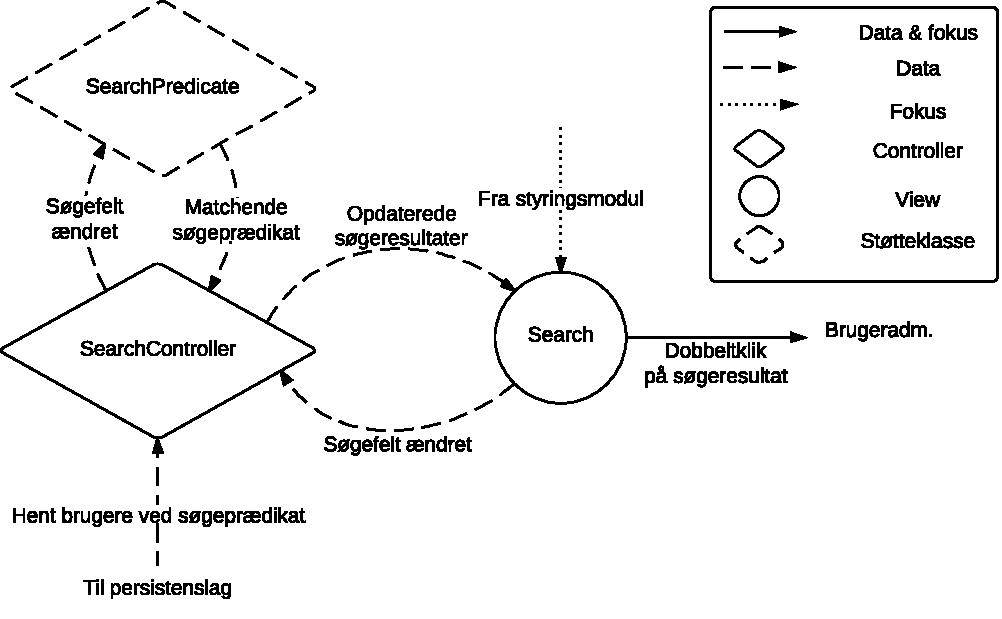
\includegraphics[width=\textwidth]{search-diagram.pdf}
  \caption{Diagram over søgemodulet} \label{fig:soegemodul}
\end{figure}

% subsection funktionalitet (end)

% subsection s_gemodul (end)
